% sddsgencontrolbits: create BPM acquisition control bits or send RAM data.
\begin{sddsprog}{sddsgencontrolbits}
\item \textbf{description:}
\verb+sddsgencontrolbits+ creates a file of BPM acquisition control
bits from unsigned-long RAM data or from command line
parameters. There is an option to send the RAM data to EPICS,
introduced originally as a secondary feature. The separate bits of
data of the output file can then be used in the {\tt tcl/tk} GUI {\tt
MpBPMWaveformViewer} for generating waveforms displays of the control
bits. It was later realized that this command tool with the EPICS
waveform writing is really useful in script-based experiments where one
or more aspect of the acquisition is modified in a systematic way.

The BPM acquisition is controlled by an array of 3888 32-bit unsigned
long integers loaded in as an EPICS waveform controls. Four BPMs can
be controlled for up to 3888 consecutive samples in a repeated
fashion.  The 32 bits control the plane, accumulator and ``use
sample'' switches for each BPM, and other global control switches. The
control bits are shown in Figure \ref{fig:acquisitionControlRam} and
explained in further detail in \cite{Norum2007}.

\begin{figure}[htb]
\centering
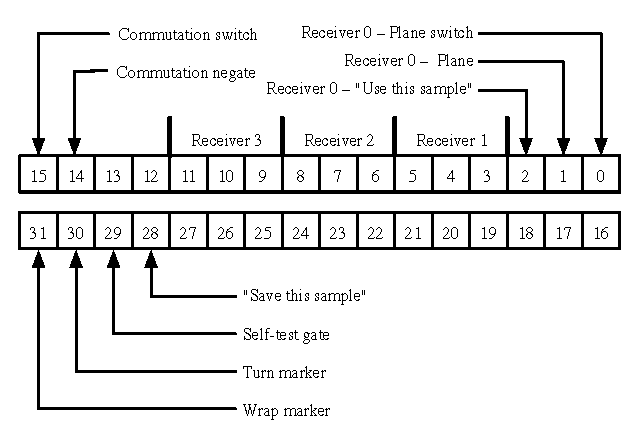
\includegraphics[width=\textwidth]{acquisitionControlRam.eps}
\caption{Acquisition control bit assignments. Courtesy of Eric Norum.}
\label{fig:acquisitionControlRam}
\end{figure}

\item \textbf{examples:}

The contents of the file {\tt controlRAM} is converted to control bits
file {\tt RAMcontrolBits}.
\begin{verbatim}
sddsgencontrolbits controlRAM RAMcontrolBits
\end{verbatim}
where the contents of the 3888-row file {\tt controlRAM} are
\begin{verbatim}
2 columns of data:
NAME            UNITS           SYMBOL          FORMAT          TYPE    FIELD  DESCRIPTION
                                                                        LENGTH
Index           NULL            NULL            NULL            long    0       NULL
Waveform        NULL            NULL            NULL            ulong   0       NULL
\end{verbatim}
and the contents of the file {\tt RAMcontrolBits} are mostly short-integer columns
\begin{verbatim}
10 columns of data:
NAME            UNITS           SYMBOL          FORMAT          TYPE    FIELD  DESCRIPTION
                                                                        LENGTH
Index           NULL            NULL            NULL            long    0       NULL
PlaneSwitch     NULL            NULL            NULL            short   0       NULL
Accumulator     NULL            NULL            NULL            short   0       NULL
CommutationNegate NULL            NULL            NULL            short   0       NULL
CommutationSwitch NULL            NULL            NULL            short   0       NULL
Sample          NULL            NULL            NULL            short   0       NULL
TurnMarker      NULL            NULL            NULL            short   0       NULL
WrapMarker      NULL            NULL            NULL            short   0       NULL
SaveSample      NULL            NULL            NULL            short   0       NULL
SelfTest        NULL            NULL            NULL            short   0       NULL
\end{verbatim}
This file {\tt RAMcontrolBits} has two data pages, one page of 3888
rows for the RAM content array, and a second data page of 4096 rows to
simulate what the FPGA transient recorder (i.e. ``scope'') would
record. This data content is the same data as in the first page, but
shifted by 2048 indices, and repeating in both directions to fill 4096
time slots. The second page seems to be superfluous, but it is needed
to produce simulated waveforms in the GUI {\tt MpBPMWaveformViewer}.

Presently the output only return data for one BPM at a time ({\tt
PlaneSwitch},{\tt Accumulator}, and {\tt Sample}) by default the BPM
in position 0 (from receiver positions 0,1,2,3). The column {\tt
Accumulator} is referred to in \cite{Norum2007} as simply ``Plane''.

\item \textbf{synopsis:}
\begin{verbatim}
usage: sddsgencontrolbits <inputRAMFile> <outputFile>
          [-setRAMWaveformPV=<string>] [-controlRAMFile=<filename>] [-comment=<string>] 
          [-receiver=0|1|2|3]

sddsgencontrolbits {-RAMWaveformPV=<string> [-scopeArrayLength=<int>] |
          -scopeWaveformPV=<string> -turnsPerWrap=<int> [-RAMArrayLength=<string>] |
          -RAMWaveformPV=<string> -scopeWaveformPV=<string> } <outputFile>
          [-setRAMWaveformPV=<string>] [-controlRAMFile=<filename>] [-comment=<string>]

sddsgencontrolbits  [-RAMArrayLength=<string>] [-scopeArrayLength=<int>] [-receiver=0|1|2|3]
          {-presetRAMconfiguration=<string>,file=<filename> |
           -planeMode=<string> -commutationMode=<string>]
           -sampleMode={single|continuous|bunchPattern=<string>}
           -bunchPatternFile=<filename> -samplesPerBunch=<int>
           -turnMarkerOffset=<int> -transitionDeadTime=<int> }
           [-scopeTriggerIndexOffset=<int>] [-receiver=0|1|2|3]
           [-setRAMWaveformPV=<string>] [-controlRAMFile=<filename>] [-comment=<string>]
           [-accumulatorMode=<string>] [-turnMarkerInterval=<integer>]
           [-secondSampleBunch=delay=<int>,samplesPerBunch=<int>]
Creates a file of RAM control bits.
Optionally writes to a RAM acquisition control waveform.
Each usage represent one of three ways to supply input data:
1) input file of RAM data,
2) RAM or scope readback waveform PV, or
3) RAM configuration parameters
such as preset bunch pattern and others.
<inputRAMFile>      file containing the values of a RAM waveform record. The data
                    is an array of unsigned long integer.

-RAMWaveformPV      RAM waveform PV name.
-scopeWaveformPV    digital scope waveform PV name.
-RAMArrayLength     the length of control RAM waveform PV needed for generating control bits from
                    bunch pattern.
-scopeArrayLength   the length of digital scope waveform PV needed for generating control bits from
                    bunch pattern.
-turnsPerWrap       number of turns in each wrap;
                    "Simulated" scope readback control bits can normally be generated
                    from RAM long integer data. However for the inverse generation the quantity 
                    turnsPerWrap is required. This option is required for the -scopeWaveformPV 
                    input method.

-presetRAMconfiguration  specifies a particular configuration from the file of RAM configuration presets.
                    A preset configuration consists of Label, PlaneMode, CommutationMode,
                    SampleMode, BunchPattern, SamplesPerBunch, TurnMarkerOffset, and TransitionDeadTime.
                    The preset string value must match one of the values of Label of the preset file.
                    The default file is /home/helios/oagData/sr/BPMcontrolRAM/presetPatterns.
                    If this option is provided, then the planeMode, commutationMode and sampleMode
                    options will be overridden.
-planeMode          the plane switch mode with values x, y, xy1, or xy2, which stands for
                    x plane, y plane, switch x/y per turn, or switch x/y every two turns.
                    (each turn has 324 time slots.)
-commutationMode    commutation switch mode with possible values of a, b, ab1, and ab2,
                    which stands for 0 degree, 180 degrees, switch between 0 and 180 every turn,
                    or switch  between 0 and 180 every two turns.
-sampleMode         sample mode with values continuous, single or pattern.
                    If "pattern" is selected, then the value of suboption bunchPattern must be given
                    and must match up with a bunch pattern defined in the preset bunch pattern file.
-bunchPatternFile   file that contains the properties of preset bunch patterns.
-accumulatorMode    accumulation switch mode; defaults to the plane mode if omitted.
-transitionDeadTime dead time length in units of timing slots for which samples will not be taken.
-turnMarkerOffset   the offset of turn marker. The first turn marker starts from this offset, and
                    the others are spaced 324 time steps.
-samplesPerBunch    number of consectuive samples to be collected per bunch. Presently it
                    is the same for all bunches.
-turnMarkerInterval turn marker interval, default is 324.
-secondSampleBunch  add a second sample bunch; delay gives the offset from the first bunch
                    and samplesPerBunch sets the number of samples.
-scopeTriggerIndexOffset  provides the offset between scope trigger and wrap marker
                    (which is normally set at 2048 by PV S42B:scope:gtr:numberPTS).

The output options are the same in the three usages.
<outputFile>        file of the separated control bits of a RAM waveform record.
                    Columns are Index, PlaneSwitch, CommutationSwitch, Sample,
                    TurnMarker, P0Marker, WrapMarker, all short integers except for Index,
                    which is long integer.
                    The digital scope readback waveform record is simulated and is
                    included as the second data page.
-setRAMWaveformPV   if provided, the control RAM long integer data will be written to this PV.
                    Note that when used with -RAMWaveformPV input with the same PVs,
                    the same values are read and written to the same PV.
-controlRAMFile     if provided, the control RAM long integer data will be written to this file.
-comment            provide comments for saving the control RAM into controlRAMFile .
-receiver           provide the receiver number to select from the control RAM when
                    creating the control bits file, which has room for only one set
                    of flags. When setting RAM all receivers have the same flags.
Program by H. Shang, ANL (EPICS 3.14.8.2, Mar 26 2007).

\end{verbatim}
\normalsize

\item \textbf{files:}
\begin{itemize}
  \item \textbf{input file:} \par
  RAM waveform record containing unsigned long integer values.
  \item \textbf{output file:} \par
  Control bits separated into individual columns; includes simulated scope readback page.
  \item \textbf{bunch pattern file:} \par
  Definitions of preset bunch patterns for pattern-based sampling modes.

  \item \textbf{switches:}
  \begin{itemize}
    \item {\tt -RAMWaveformPV} --- RAM waveform PV name.
    \item {\tt -scopeWaveformPV} --- digital scope waveform PV name.
    \item {\tt -planeMode} --- plane switch mode for receivers.
    \item {\tt -accumulatorMode} --- accumulation switch mode.
    \item {\tt -commutationMode} --- commutation switch mode.
    \item {\tt -sampleMode} --- sampling mode, including bunch patterns.
    \item {\tt -bunchPatternFile} --- file of preset bunch patterns.
    \item {\tt -samplesPerBunch} --- samples collected per bunch.
    \item {\tt -secondSampleBunch} --- add delayed second sample bunch.
    \item {\tt -turnMarkerOffset} --- offset to first turn marker.
    \item {\tt -turnMarkerInterval} --- interval between turn markers.
    \item {\tt -transitionDeadTime} --- dead time in timing slots.
    \item {\tt -RAMArrayLength} --- length of control RAM waveform PV.
    \item {\tt -scopeArrayLength} --- length of scope waveform PV.
    \item {\tt -turnsPerWrap} --- number of turns per wrap for scope data.
    \item {\tt -scopeTriggerIndexOffset} --- offset between scope trigger and wrap marker.
    \item {\tt -setRAMWaveformPV} --- write control RAM data to this PV.
    \item {\tt -controlRAMFile} --- write control RAM data to this file.
    \item {\tt -comment} --- comment string saved with control RAM data.
    \item {\tt -receiver} --- select receiver when creating control bits (obsolete).
  \end{itemize}
\end{itemize}

\item \textbf{see also:}
\begin{itemize}
  \item \progref{sddsexperiment}
\end{itemize}
\item \textbf{author:} Louis Emery, Hairong Shang, Robert Soliday, ANL/APS.
\end{sddsprog}
